\documentclass[12pt]{report}

\usepackage{mathptmx}
\usepackage{graphicx}
\usepackage{hyperref}
\usepackage{amsmath}
\usepackage{ amssymb }
\usepackage{setspace}
\usepackage{booktabs}
\usepackage{rotating}
\usepackage{makecell}

\usepackage{xcolor}
\hypersetup{
    colorlinks,
    linkcolor={red!50!black},
    citecolor={purple!50!black},
    urlcolor={blue!80!black}
}

\usepackage{titlesec}
\titleformat{\chapter}[hang]
{\bfseries\Huge}{\chaptertitlename\ \thechapter:}{16pt}{\Huge}
\titleformat{\section}
  {\Large\bfseries}{\thesection}{14pt}{}
\titleformat{\subsection}
  {\large\bfseries}{\thesubsection}{11pt}{}
  
  
\usepackage[font=small,labelfont=bf,textfont=bf]{caption}
%\newcommand{\cchapter}[1]{\chapter[#1]{\centering #1}}
\usepackage[top=1.0in,bottom=1.0in,left=1.0in,right=1.0in]{geometry} 

\usepackage{pdfpages}

\begin{document}
\includepdf[pages={1}]{certi.pdf}

\begin{spacing}{1.5}
\chapter{Introduction}

% NN has become defacto standard for NLP models
Machine Learning based methods have become a de facto standard for solving majority of Natural Language Processing problems. 
With the increase in complexity of models, it has become difficult to test and debug to see if they are robust for deployment.
The standard metrics for model evaluation are measured by averaging error over a testing dataset which is kept separate from training data.
While these metrics, like accuracy, are useful, developers can overestimate their models generalization capabilites as testing data is obtained in same manner like training data.
A  model can show impressive perfomance over these metrics, but it might be due to superficial cues which happens to be predictive most of the time \cite{jia2019}.

Recent research has shown that Complex models for Natural Language Processing are prone to ``brittleness'' i.e. ``different ways of phrasing the same sentence can often cause the model to output different predictions'' \cite{riberio2018}.
Moreover, NLP models are vulnerable to small changes in input \textit{(oversenstivity)}, called Adversarial pertrubations, which leads them to produce wrong output \cite{liang2018}.
The changes are small enough that it appears as same sentence semtanically (also syntactically in some case) to a human but causes ML model to mispredict.

In real world scenario, adversarial examples can be used to evaluate if deeper, intelligent patterns are recognized by the model so that it generalizes well and is robust.
Using these attacks, we can understand our model's capabilities and limitations, and, as a longstanding problem in AI, check true language understanding and reasoning abilities.
In addition, since an adversarial attack changes the output of a model, it poses security concerns. It can be used to exploit the model, for example, a spammer can generate adversarial pertrubations to evade a spam filter or evade a False news detector.
Hence, our objective for adversarial attacks is twofold: \textit{model evaluation and interpretation}, and \textit{exposing system vulnerability}.

There are several ways to generate adversarial examples but we are interested in \textbf{Universal Adversarial Triggers} that can be applied on any input sequence in the domain.
These are input independent sequence of tokens, which, when concatenated with input text, fools NLP models to mispredict. Since these tokens are input-agnostic, they pose a bigger threat that input-specific pertrubations, as they can be ditributed to a large number and they work on majority of inputs. Additional, global model behaviour insights can be drawn upon by universal triggers \cite{wallace2019}. In the project, we try to generate universal adversarial triggers for Text Classification NLP task.
% about UNiversal triggers

\section{Text Classification}
Text Classification is a categorization problem in which a text, sentence, or documents is assigned a predefined tag according to its content. It is one of the fundamental problem in Natural Language Processing which can be solved with various techniques like \textit{knowledge based methods, statical methods}, and other hybrid techniques.
Some real world examples of Text classification includes:
\begin{enumerate}
\item Spam Filters
\item Categorizing News articles and movie genre
\item Sentiment analysis or Opinion mining
\end{enumerate}
We demonstrate the effectiveness of adversarial examples using \textbf{Sentiment Analysis} classifier.

\section{Adversarial examples}
% Show CV example maybe

Adversarial example for text classification can be formally defined as follows:
Consider $f$ as a classifier function which classifies input $s \in S$ to one of the class $c \in C$, then $s'$ is an adversarial example if $s'$ is recognized in the same class $c$ by a Human observer, but $f(s) \neq f(s')$.

\subsection{Choice of adversarial examples: Granularity}
To generate adversarial example, we need a small ``change'' than can transform $s$ to $s'$. This change, in case of NLP, can be at following levels or granularity: \textit{character, words} and \textit{ sentence}.
\paragraph{Character Level}
At this granularity, the aim is to change characters of a word in order to generate small difference to have adversarial effect. Characters could be removed, added, or replaced to produce the change.
% TODO Add pros and cons
Fig. \ref{ebrahimi_word} shows character level changes that causes misclassification.
\begin{figure}[!h]
  \centering
  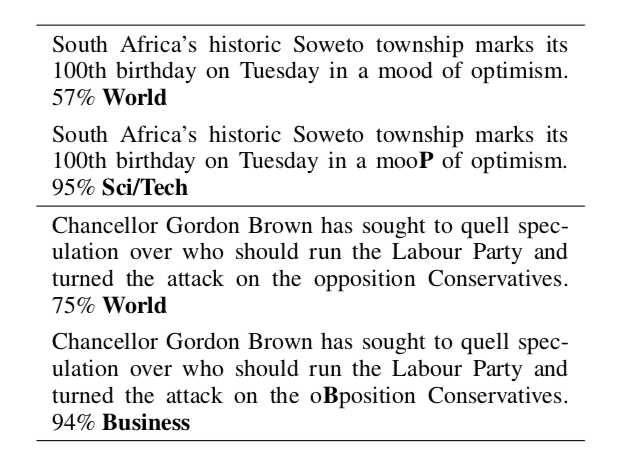
\includegraphics[width=0.5\linewidth]{./img/ebrahimi_char.png}
  \caption{Character level change \cite{ebrahimi2018}}
  \label{ebrahimi_word}
\end{figure}

\paragraph{Word Level}
At this granularity, the aim is to replace a word with a similar word to generate adversarial example. New words can also be added or existing words can be removed to bring the change.
% TODO add pros and cons
Fig. \ref{alzantot_senti} shows an word level adversarial example created by Alzantot et al. \cite{alzantot2018}.
\begin{figure}[!h]
  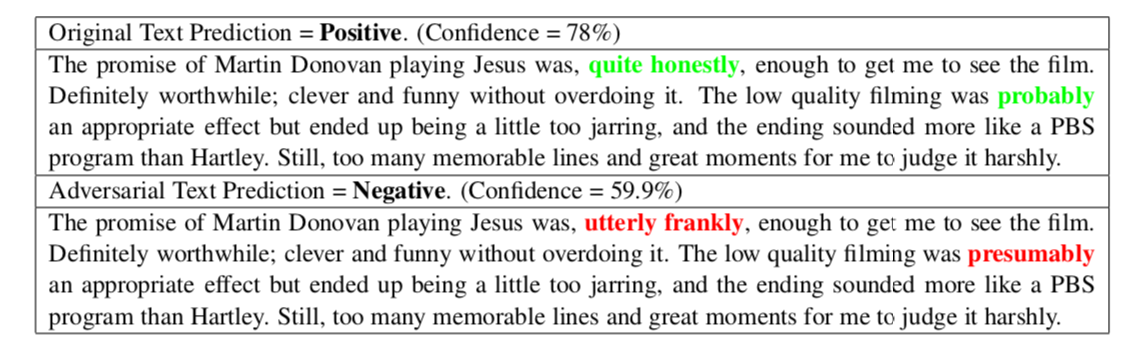
\includegraphics[width=\linewidth]{./img/alzantot_senti.png}
  \caption{Word level change \cite{alzantot2018}}
  \label{alzantot_senti}
\end{figure}

\paragraph{Senetence Level}
At this level, an adversarial example is created by paraphrasing the sentence, by removing a sentence, or by appending a new sentence, such that the meaning of the document remains the same as before.
% TODO add pros and cons
Fig. \ref{liang_sen} shows how addition of sentence causes model to misclassify text form \textit{Album} to \textit{Company}.

\begin{figure}[!h]
  \centering
  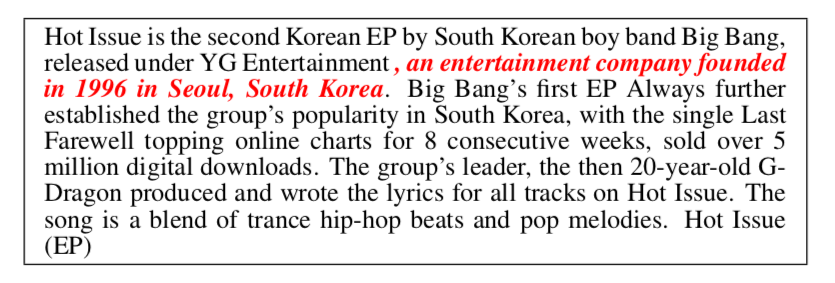
\includegraphics[width=0.8\linewidth]{./img/liang_sen.png}
  \caption{Sentence level change. 99.9\% \textit{Album} to 94.0\% \textit{Company} \cite{liang2018}}
  \label{liang_sen}
\end{figure}

\subsection{Universal Adversarial triggers}
In Universal Adversarial triggers, we search for pertrubations at word level.
We try to find input-agnostic words that can be inserted in original sentence.
More specifically, we want a sequence of words $w$ that can be concatenated to input $s$ belonging to probablity distribution $P(L)$ that causes classifer $f$ to mispredict.
Hence, our adversarial example $s'$ will be of the form:
\begin{equation}
  \label{adv_s}
  s' = w \oplus s = s_i...s_k | w_1...w_m | s_{k+1}...s_j; \; (i,j) \in [0, len(s)] 
\end{equation}

To get the value or $w$, we maximize the classifier loss over all dataset. If true output is $y$, then the optimization needed to be solved is,
\begin{equation}
  \label{eq: optim}
  \hat{w} = \underset{w}{argmax} \; \mathcal{E}_{s \sim P(L)}[\mathcal{L}(y, f(s'))]
\end{equation}
Since we are optimizing the expected loss with respect to the
data distribution, the resulting sequence $\hat{w}$ would ideally be
universal. We constrain equation \ref{adv_s} to insert adversarial triggers at the beginning of the sentence. Hence, out $s'$ becomes:
\begin{equation}
  \label{eq: trigger}
  s' = w \oplus s = w_1...w_m \cdot s_1...s_n
\end{equation}

\chapter{Process Flow Diagram}

\chapter{Output}
\cite{behjati2019}
\end{spacing}

\bibliography{report}
\bibliographystyle{ieeetr}

\end{document}
